\documentclass[12pt,fleqn]{article}\usepackage{../common}
\begin{document}
Kisitli Boltzmann Makinalari (Restricted Boltzmann Machines -RBM-)

Bir RBM icinde ikisel (binary) degerler tasiyan gizli (hidden) $h$
degiskenler, ve yine ikisel gorunen (visible) degiskenler $v$ vardir. $Z$
aynen once gordugumuz Boltzman Makinalarinda (BM) oldugu gibi normalizasyon
sabitidir.

$$ p(x,h;W) = \exp (-E(x,h)) / Z $$

$E$ tanimina ``enerji'' olarak ta atif yapilabiliyor.

$$ E(x,h) = -h^TWx - c^Tx - b^Th $$

BM'lerden farkli olarak RBM taniminda $c,b$ degiskenleri var. Bu
degiskenler yanlilik (bias) icin, yani veri icindeki genel egilimi
saptamalari icin modele konulmustur. Ayrica $h^TWx$ terimi var, bu BM'deki
 $x^TWx$ biraz farkli, gizli degiskenler, $h$ uzerinden $x$'ler arasinda
baglanti yapiyor. Bir baska ilginc farklilik BM ile tum $x$ ogeleri
birbirine baglanabiliyordu, RBM ile daha az (ya da fazla) olabilecek $h$
katmaninda baglantilar paylasiliyor. Ozellikle azaltma durumunda RBM
ozellik alanini azaltarak bir tur genellemeyi gerceklestirebiliyor.

Formul alttaki gibi de acilabilir,

$$ = - \sum_j \sum_k W_{j,k}h_jx_k - \sum_k c_kx_k - \sum_j b_jh_j  $$

RBM'lerin alttaki gibi resmedildigini gorebilirsiniz.

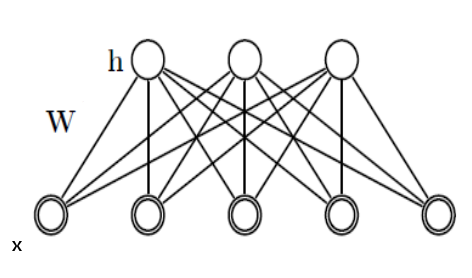
\includegraphics[height=4cm]{rbm_01.png}
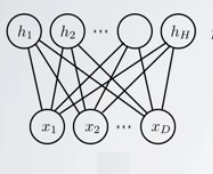
\includegraphics[height=4cm]{rbm_02.png}

$h,x$ degiskenleri olasilik teorisinden bilinen rasgele degiskenlerdir,
yani hem $x$'e hem de $h$'e ``zar attirabiliriz'' / bu degiskenler
uzerinden orneklem toplayabiliriz. 

Ayrica, RBM'ler aynen BM'ler gibi bir olasilik yogunluk fonksiyonu
uzerinden tanimlanirlar, onceki formulde gordugumuz gibi, tum mumkun
degerleri uzerinden entegralleri (ya da toplamlari) alininca sonuc 1 olur,
vs.

RBM'lerin ``kisitli'' olarak tanimlanmalarinin sebebi gizli degiskenlerin
kendi aralarinda, ve gorunen degiskenlerin kendi aralarinda direk
baglantiya izin verilmemis olmasidir, bu bakimdan
``kisitlanmislardir''. Baglantilara, $W$ uzerinden sadece gizli ve gorunen
degiskenler (tabakalar) arasinda izin verilmistir. Bu tabii ki matematiksel
olarak bazi kolayliklar sagliyor.

Devam edelim, ana formulden hareketle cebirsel olarak sunlar da dogrudur,

$$ p(x,h;W) = \exp (-E(x,h)) / Z $$

$$ 
\mlabel{2}
= \exp (h^TWx + c^Tx + b^Th ) / Z $$

$$ = \exp (h^TWx) \exp (c^Tx) \exp(b^Th) / Z $$

cunku bir toplam uzerindeki $\exp$, ayri ayri $\exp$'lerin carpimi
olur. Ayni mantikla, eger ana formulu matris / vektor yerine ayri
degiskenler olarak gormek istersek,

$$ 
p(x,h;W) = \frac{1}{Z}
\prod_j \prod_k \exp (W_{jk}h_jx_k) \prod_k \exp(c_kx_k) \prod_j \exp(b_jh_j) 
 $$

Notasyonu kolaylastirmak amaciyla $b,c$ terimlerini $W$ icine absorbe
edebiliriz, $x_0=1$ ve $h_0=1$ degerlerini mecbur tutarsak ve $w_{0,:}=c$
ve $w_{:,0}=b$ dersek, yani $W$'nin sifirinci satirinin tamamini $c$'ye set
edip, sifirinci kolonunun tamamini $b$'ye set edersek, RBM ana formulunu
tekrar elde etmis oluruz, fakat artik 

$$ E(x,h) = -h^TWx $$


$$ = - \sum_j \sum_k W_{j,k}h_jx_k  $$

ve

$$ p(x,h;W)  = \exp (h^TWx) / Z $$

yeterli olacaktir. Bir diger kolaylik $x,h$ yerine tek degisken kullanmak,

Eger $y \equiv (x,h)$ olarak alirsak, 


$$ P(x,h;W) = \frac{1}{Z(W)} \exp 
\bigg[ 
\frac{1}{2} y^T W y
\bigg]
$$

Aslinda acik konusmak gerekirse ``enerji'' gibi kavramlarla ugrasmak, ya da
icinde eksi terimler iceren bir grup degiskenin tekrar eksisini almak ve
eksilerin etkisinin notralize etmis olmak yerine bastan (2)'deki ifadeyle
yola cikmak daha kisa. Giristeki aciklamalari literaturde gorulebilecek
bazi anlatimlari aciklamak icin yaptik. 

Neyse, $h$ uzerinden marjinalize edersek,

$$ P(x;W) = \sum_h \frac{1}{Z(W)} \exp 
\bigg[ 
\frac{1}{2} y^T W y
\bigg]
$$


$$  
\mlabel{1}
P(x;W) = \frac{1}{Z(W)}  \sum_h \exp 
\bigg[ 
\frac{1}{2} y^T W y
\bigg]
$$


Ve $Z(W)$ 

$$ Z(W) = \sum_{h,x} \exp 
\bigg[ 
\frac{1}{2} y^T W y
\bigg]
$$

(1) denkleminde bolumunden sonraki kisma $Z_x(W)$ dersek, sanki ayni $\exp$
denkleminin ``farkli bir sekilde marjinalize edilmis hali'' olarak
gostermis oluruz onu, ve boylece daha kisa bir formul kullanabiliriz,

$$  
P(x;W) = \frac{1}{Z(W)}  
\underbrace{
\sum_h \exp 
\bigg[ 
\frac{1}{2} y^T W y
\bigg]
}_{Z_x(W)}
$$

O zaman 

$$  
P(x;W) = \frac{Z_x(W)}{Z(W)} 
$$

elde ederiz. Veri uzerinden maksimum olurluk icin, yine log uzerinden bir
hesap yapariz, BM icin yapmistik bunu,

$$  
\mathcal{L} = 
\ln \big( \prod_{n=1}^{N} P(x^{n};W) \big) = 
\sum_{n=1}^{N} \ln P(x^{n};W) 
$$

$$ 
= \sum_{n=1}^{N} \ln \frac{Z_{x^{(n)}}(W)}{Z(W)}  
= \sum_{n=1}^{N}  \big(\ln Z_{x^{(n)}} - \ln Z \big) 
$$

$$ 
\mlabel{3}
\frac{\partial \mathcal{L} }{\partial w_{ij}} = 
 \sum_{n=1}^{N}  \big( \frac{\partial \ln Z_{x^{(n)}} }{\partial w_{ij}}
- \frac{\partial \ln Z }{\partial w_{ij}} \big)
$$

Parantez icindeki 1. turevi alalim,

$$ 
\frac{\partial \ln Z_{x^{(n)}} }{\partial w_{ij}} = 
\frac{\partial }{\partial w_{ij}}  
\ln \bigg[ 
\sum_h \exp \big( \frac{1}{2} y^{n^T} W y^n \big) 
\bigg]
$$

$$ 
= \frac{1}{Z_{x^{(n)}}}  \bigg[ \sum_h \frac{\partial }{\partial w_{ij}} \exp \big( \frac{1}{2} y^{n^T} W y^n  \big) \bigg]
$$

$$ 
= \frac{1}{Z_{x^{(n)}}}  
\bigg[ 
\sum_h  \exp \big( \frac{1}{2} y^{n^T} W y^n  \big) 
\frac{\partial }{\partial w_{ij}} y^{n^T} W y^n 
\bigg]
$$

$$ 
= \frac{1}{Z_{x^{(n)}}}  \sum_h  \exp \big( \frac{1}{2} y^{n^T} W y^n  \big) y_iy_j
$$


$$ 
= \sum_h  \frac{1}{Z_{x^{(n)}}}  \exp \big( \frac{1}{2} y^{n^T} W y^n  \big) y_iy_j
$$

$Z_{x^{(n)}}$'nin ne oldugunu hatirlarsak, $\exp$ ifadesinin $h$ uzerinden
marjinalize edilmis hali,

$$ 
= \sum_h  \frac{\exp \big( \frac{1}{2} y^{n^T} W y^n  \big)}
{\sum_h \exp \big( \frac{1}{2} y^T W y \big) } 
y_iy_j
$$

Eger bolumun ustunu ve altini $Z$ ile bolsek,

$$ 
= \sum_h  
\frac{\exp \big( \frac{1}{2} y^{n^T} W y^n  \big) / Z} 
{\sum_h \exp \big( \frac{1}{2} y^T W y \big) / Z} 
y_iy_j
$$

Ust kisim $P(y;W)$ yani $P(x,h;W) $ alt kisim $P(x;W)$ olmaz mi? Evet! Ve,


$$ P(h|x^n;W) = \frac{P(x^n,h;W)}{P(x^n;W)}  $$

olduguna gore, 

$$ =  \sum_h P(h|x^n;W) y_iy_j $$

elde ederiz. Bunu da $<y_iy_j>_{P(h|x^n;W)}$ olarak yazabiliriz. 

Simdi parantez icindeki 2. turevi alalim, yani $\frac{\partial \ln Z }{\partial w_{ij}} $,

$$ 
\frac{\partial \ln Z }{\partial w_{ij}}  = 
\sum_{h,x} \frac{1}{Z}  \exp \big( \frac{1}{2} y^{n^T} W y^n  \big) y_iy_j =
\sum_{h,x} P(y^n;W)  y_iy_j
$$

ki bu son ifadeyi de $<y_iy_j>_{P(y^n;W)}$ olarak yazabiliriz. Tamamini,
yani (3) ifadesini, artik soyle yazabiliriz,

$$
\sum_{n=1}^{N}  \big( \frac{\partial \ln Z_{x^{(n)}} }{\partial w_{ij}} - \frac{\partial \ln Z }{\partial w_{ij}} \big)
= \sum_{n=1}^{N}  <y_iy_j>_{P(h|x^n;W)} - <y_iy_j>_{P(y^n;W)}
$$





















\end{document}
